%!TeX TS-program=arara
% arara: lualatex
% arara: lualatex
\PassOptionsToPackage{pdfencoding=auto}{hyperref}
\documentclass[aspectratio=169]{beamer}

\usepackage[ngerman]{babel}
\usetheme{FSU}
\beamertemplatenavigationsymbolsempty
\usetikzlibrary{positioning,calc,arrows.meta,shapes.geometric}

\title[Blind Spot]{Blind Spot}
\subtitle[Stand M1]{Hinderniswarner für Blinde: Stand zu Meilenstein M1}
\author[Köllmann \& Brückner]{Yannik Köllmann \& Mika Brückner}
\institute[Intelligente Systeme]{Anwendungspraktikum 3D-Rechnersehen, WiSe 2026/27}
\date{25.\,November 2026}

% Modellgruppen wie in den Abbildungen: blau = Brennweite, orange = keine Kamerainfo, grün = relativ
\definecolor{gfocal}{HTML}{2874D6}
\definecolor{gnocam}{HTML}{EC6A36}
\definecolor{grel}{HTML}{17AF7C}

\newcommand{\tile}[3]{% Farbe, Titel, Text
  \begin{tcolorbox}[enhanced,frame hidden,sharp corners=all,colback=#1!12,
      coltext=cdhausfarbe,left=.2cm,right=.2cm,top=.15cm,bottom=.15cm,
      borderline west={1.2mm}{0pt}{#1}]
    {\bfseries #2}\par\smallskip #3
  \end{tcolorbox}}

\begin{document}

\begin{frame}[plain,noframenumbering]
  \titlepage
\end{frame}

% ---------------------------------------------------------------- Projekt
\section{Das Projekt}
\begin{sframe}
  \begin{itemize}
    \item iPhone-Kamera auf Brusthöhe, \textbf{monokulare Tiefenschätzung}, Warnung als \textbf{Stereo-Ton}.
    \item Das Basismodell steht noch nicht fest: Wir vergleichen erst, dann entscheiden wir.
  \end{itemize}
  \vspace{.3cm}
  \centering
  \begin{tikzpicture}[font=\small,
      pstep/.style={draw=none,text=white,align=center,minimum width=2.55cm,minimum height=1.5cm,
                   inner sep=4pt,text width=2.35cm},
      arr/.style={->,thick,cdhausfarbe}]
    \node[pstep,fill=cdbiowiss] (s1) {Bild\\\scriptsize Brustkamera};
    \node[pstep,fill=cdbiowiss,right=.3cm of s1] (s2) {Tiefe\\\scriptsize 14 Modelle verglichen};
    \node[pstep,fill=cdhausfarbe!35,right=.3cm of s2] (s3) {Bodenskalierung\\\scriptsize WP 2.2};
    \node[pstep,fill=cdwiwiss,right=.3cm of s3] (s4) {Korridor-Alarm\\\scriptsize WP 3.1, ungemessen};
    \node[pstep,fill=cdhausfarbe!35,right=.3cm of s4] (s5) {Stereo-Ton\\\scriptsize Echtzeit, App};
    \foreach \a/\b in {s1/s2,s2/s3,s3/s4,s4/s5}{\draw[arr] (\a) -- (\b);}
    \node[draw=none,fill=cdbiowiss,minimum size=.25cm] (l1) at (.3,-1.5) {};
    \node[anchor=west,font=\scriptsize] at (l1.east) {läuft offline};
    \node[draw=none,fill=cdwiwiss,minimum size=.25cm] (l2) at (3.3,-1.5) {};
    \node[anchor=west,font=\scriptsize] at (l2.east) {gebaut, noch nicht gemessen};
    \node[draw=none,fill=cdhausfarbe!35,minimum size=.25cm] (l3) at (8.1,-1.5) {};
    \node[anchor=west,font=\scriptsize] at (l3.east) {offen};
  \end{tikzpicture}
\end{sframe}

% ---------------------------------------------------------------- Stand
\section{Stand des Projekts}
\begin{sframe}
  \begin{minipage}[t]{.48\textwidth}
    \vspace{0pt}
    \tile{cdsozialwiss}{Daten}{\small SANPO (40 annotierte Testbilder) und 14 eigene iPhone-Sequenzen mit LiDAR-Tiefe, Tag und Nacht, drinnen und draußen.}
  \end{minipage}\hfill
  \begin{minipage}[t]{.48\textwidth}
    \vspace{0pt}
    \tile{cdhausfarbe}{Auswertungs-Framework}{\small Ein Befehl vergleicht beliebige Modelle: Tiefenfehler je Distanz, Latenz, Speicher, Alarm-Metriken. 62 Tests in der CI.}
  \end{minipage}
  \vspace{.2cm}

  \begin{minipage}[t]{.48\textwidth}
    \vspace{0pt}
    \tile{cdphysik}{Modellvergleich}{\small 14 Modelle hinter einem Interface, in drei Gruppen: metrisch ohne Kamerainfo, metrisch mit Brennweite, relativ (528 Bilder).}
  \end{minipage}\hfill
  \begin{minipage}[t]{.48\textwidth}
    \vspace{0pt}
    \tile{cdwiwiss}{Warnlogik}{\small Korridor 0,9\,m breit, Alarm links/Mitte/rechts bei Punkten unter 3\,m, plus naive Baseline. Güte noch nicht gemessen.}
  \end{minipage}
\end{sframe}

% ---------------------------------------------------------------- Erkenntnis 1
\section{Erkenntnis: Skala ist das Problem}
\begin{sframe}
  \begin{minipage}[c]{.5\textwidth}
    \centering
    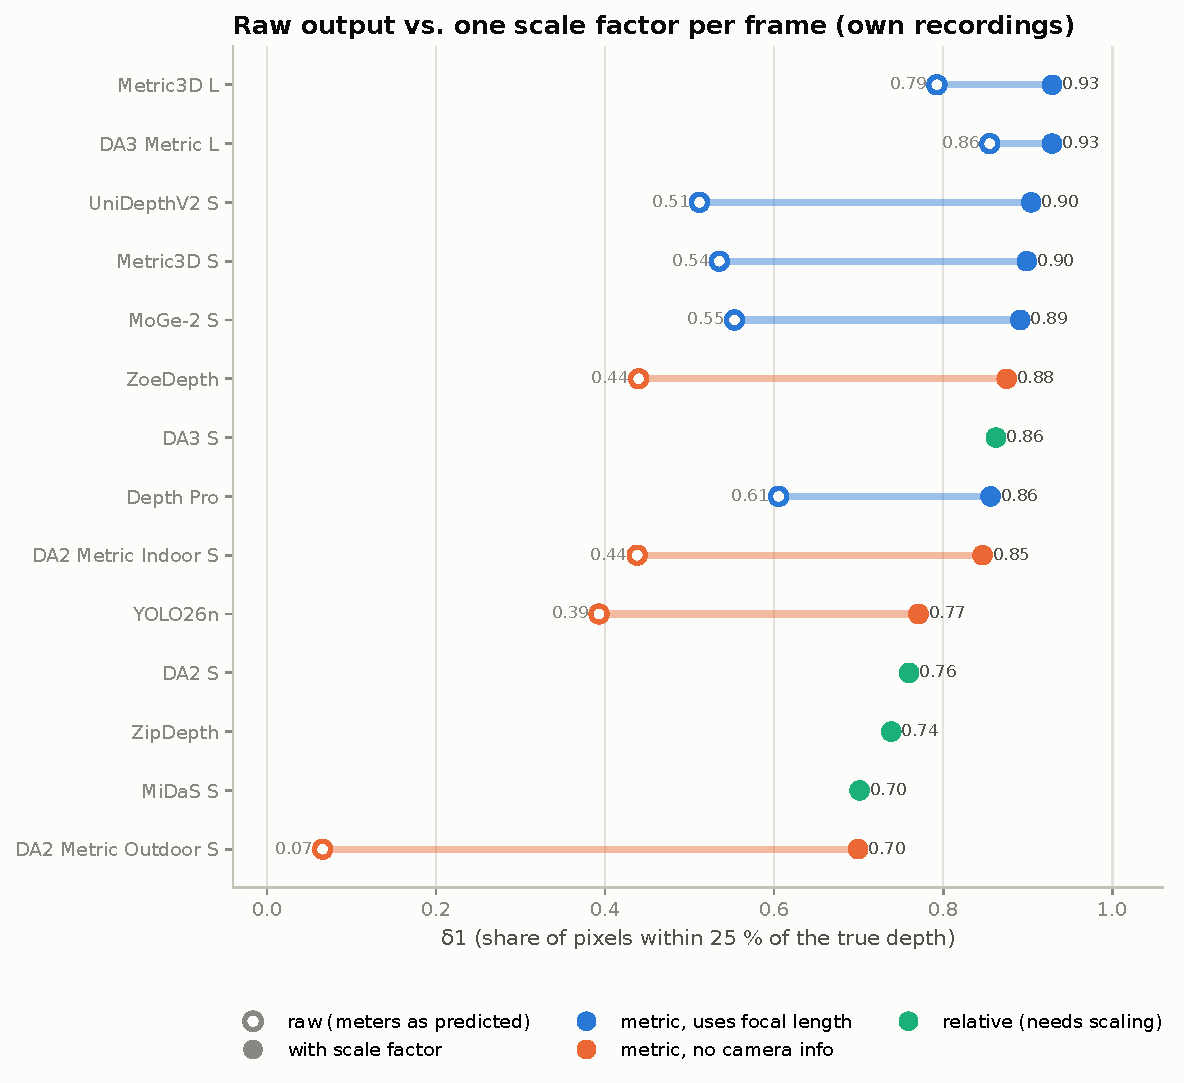
\includegraphics[height=6.1cm]{img/iphone_raw_vs_scaled.pdf}
  \end{minipage}\hfill
  \begin{minipage}[c]{.47\textwidth}
    \begin{itemize}\setlength\itemsep{4pt}
      \item Ohne Hilfe erreichen die kleinen Modelle nur $\delta_1 = 0{,}39$ bis $0{,}55$.
      \item Mit \textbf{einem richtigen Skalenfaktor pro Bild} sind es $0{,}85$ bis $0{,}90$.
      \item Die Struktur stimmt, die Meter nicht. Die geplante \textbf{Bodenskalierung (WP 2.2)} ist der wichtigste nächste Schritt.
    \end{itemize}
    {\scriptsize Der Skalenfaktor ist ein Orakel und damit eine obere Schranke.}
  \end{minipage}
\end{sframe}

% ---------------------------------------------------------------- Erkenntnis 2
\section{Erkenntnis: Genauigkeit gegen Latenz}
\begin{sframe}
  \begin{minipage}[c]{.64\textwidth}
    \centering
    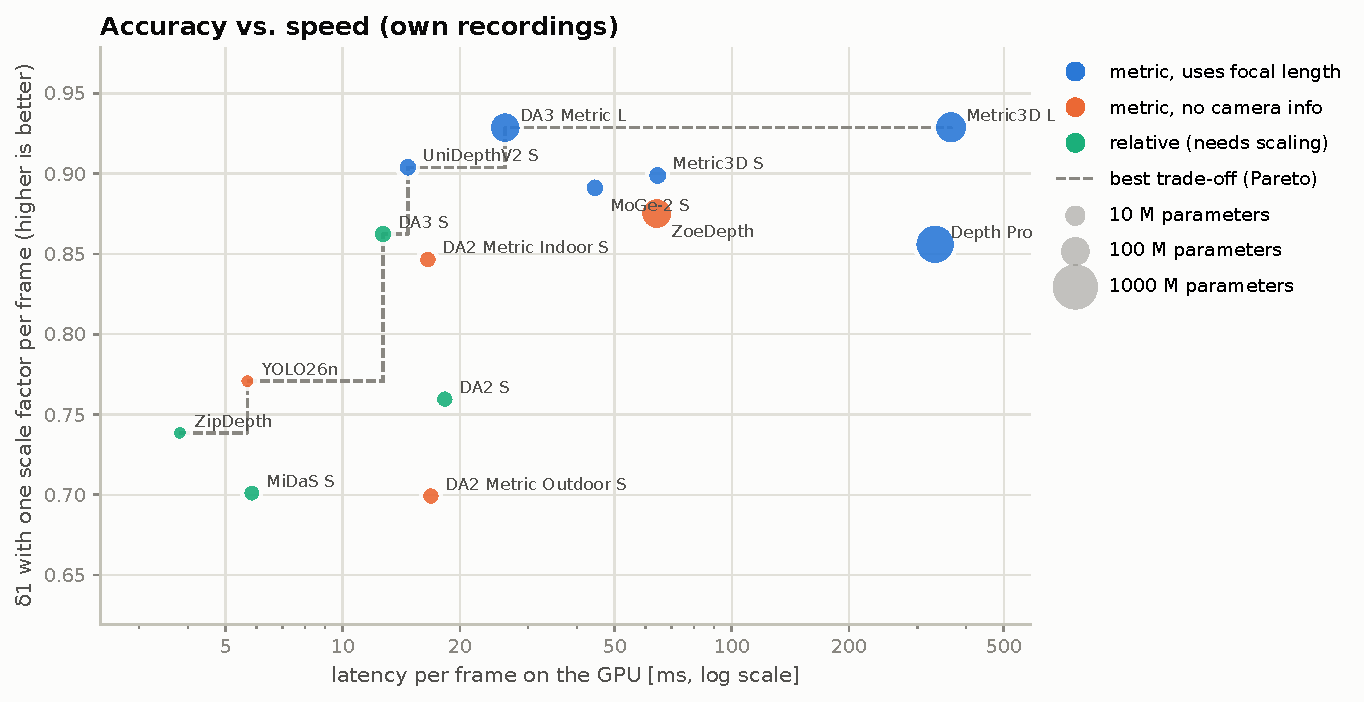
\includegraphics[width=\textwidth]{img/iphone_accuracy_vs_latency.pdf}
  \end{minipage}\hfill
  \begin{minipage}[c]{.34\textwidth}
    \footnotesize
    \textbf{Weiter in WP 2.2:}
    \begin{itemize}\setlength\itemsep{2pt}
      \item UniDepthV2 S: $\delta_1 = 0{,}90$ bei 15\,ms
      \item DA2 Metric Indoor S
      \item DA2 Small
    \end{itemize}
    \textbf{Referenz und möglicher Teacher (WP 2.3):} Depth Anything 3 Metric Large, am genauesten (0,93), aber 334\,M Parameter, zu groß fürs Handy.\par
    \vspace{.1cm}
    {\scriptsize RTX 5070 Ti, eigene Aufnahmen}
  \end{minipage}
\end{sframe}

% ---------------------------------------------------------------- Weitere Erkenntnisse
\section{Weitere neue Erkenntnisse}
\begin{sframe}
  \begin{minipage}[t]{.48\textwidth}
    \vspace{0pt}
    \tile{cdmedizin}{Nahbereich ist die Schwachstelle}{\small Alle Modelle sind unter 1\,m am schlechtesten, genau dort, wo gewarnt wird. SANPO kann das nicht messen (Stereo ab ca.\,2\,m).}
  \end{minipage}\hfill
  \begin{minipage}[t]{.48\textwidth}
    \vspace{0pt}
    \tile{cdwiwiss}{Licht zählt mehr als Innen/Außen}{\small Nachts fällt $\delta_1$ von Metric3D S von $0{,}93$ auf $0{,}83$. Getrennte Indoor- und Outdoor-Modelle würden nichts bringen.}
  \end{minipage}
  \vspace{.2cm}

  \begin{minipage}[t]{.48\textwidth}
    \vspace{0pt}
    \tile{cdsozialwiss}{Auswertung ändert das Ranking}{\small Relative Modelle brauchen Skala \emph{und} Verschiebung: DA2 Small $0{,}76$ mit einem Faktor, $0{,}94$ mit beidem.}
  \end{minipage}\hfill
  \begin{minipage}[t]{.48\textwidth}
    \vspace{0pt}
    \tile{cdbiowiss}{Jede Datenquelle gegen echte Daten prüfen}{\small iPhone-Videos liefern ein Bild weniger als Tiefenkarten: Das erste fehlte, Bild und Tiefe wären um eins verschoben gewesen.}
  \end{minipage}
\end{sframe}

% ---------------------------------------------------------------- Ausblick
\section{Stand und nächste Schritte}
\begin{sframe}
  \begin{minipage}[t]{.48\textwidth}
    \vspace{0pt}
    \textbf{Nächste Schritte (M2: 09.12.)}
    \begin{itemize}\setlength\itemsep{2pt}\small
      \item Bodenskalierung für die drei Kandidaten (WP 2.2)
      \item Eigene Aufnahmen annotieren, damit Alarme messbar werden
      \item Echtzeitbetrieb mit Audio-Feedback
      \item Modelle aufs iPhone exportieren und dort messen
      \item Echte Gehwege aufnehmen
    \end{itemize}
  \end{minipage}\hfill
  \begin{minipage}[t]{.48\textwidth}
    \vspace{0pt}
    \textbf{Risiken und offene Punkte}
    \begin{itemize}\setlength\itemsep{2pt}\small
      \item LiDAR nur bis ca.\,5\,m zuverlässig, der Fernbereich bleibt unbelegt
      \item Ob das Wunschmodell aufs Handy passt, ist offen
    \end{itemize}
  \end{minipage}
\end{sframe}

\begin{standoutframe}
  Fragen?
\end{standoutframe}

\end{document}
